\begin{figure}[tb]
\centering
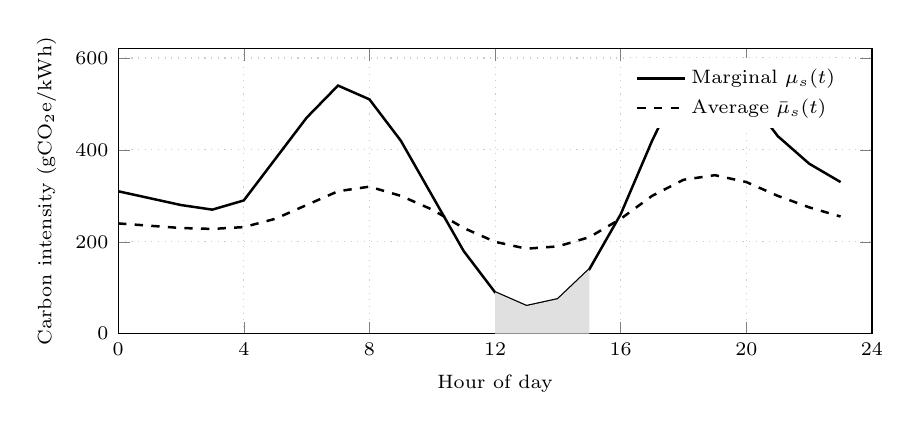
\begin{tikzpicture}
\begin{axis}[
  width=0.92\columnwidth, height=5.2cm,
  xlabel={Hour of day}, ylabel={Carbon intensity (gCO\textsubscript{2}e/kWh)},
  xmin=0, xmax=24, ymin=0, ymax=620,
  xtick={0,4,8,12,16,20,24},
  legend pos=north east, legend style={font=\scriptsize, draw=none},
  legend cell align=left,
  grid=both, grid style={dotted, black!20},
  tick label style={font=\scriptsize}, label style={font=\scriptsize},
  every axis plot/.append style={line width=0.9pt}
]
% Marginal intensity: sharp peaks at fossil ramp hours, deep troughs at solar surplus
\addplot[black, mark=none] coordinates {
 (0,310)(1,295)(2,280)(3,270)(4,290)(5,380)(6,470)(7,540)(8,510)
 (9,420)(10,300)(11,180)(12,90)(13,60)(14,75)(15,140)(16,260)
 (17,420)(18,560)(19,590)(20,520)(21,430)(22,370)(23,330)
};
% Average intensity: smoother, lags marginal, never as deep or as high
\addplot[black, dashed, mark=none] coordinates {
 (0,240)(1,235)(2,230)(3,228)(4,232)(5,250)(6,280)(7,310)(8,320)
 (9,300)(10,270)(11,230)(12,200)(13,185)(14,190)(15,210)(16,250)
 (17,300)(18,335)(19,345)(20,330)(21,300)(22,275)(23,255)
};
% Shaded surplus window 12:00-15:00
\addplot[fill=black!12, draw=none] coordinates {
 (12,0)(12,90)(13,60)(14,75)(15,140)(15,0)
} \closedcycle;
\legend{Marginal $\mu_s(t)$, Average $\bar\mu_s(t)$}
\end{axis}
\end{tikzpicture}
\caption{Marginal versus average carbon intensity over a representative
day (mock trace, calibrated to the divergence reported in
prior measurement work). The shaded band marks a renewable-surplus
window where marginal intensity drops well below the average. A
scheduler on the average signal defers into hours 10--12, where the
average is low but the marginal generator is still fossil; a scheduler
on the marginal signal defers into the shaded window, where the
incremental electron is genuinely clean. The gap between the two curves
is the carbon saving \textsc{CarbonShift} recovers.}
\label{fig:marginal-vs-avg}
\end{figure}
